% document style header
\documentclass[a4paper, 12pt]{config/homework}

% import default packages
\usepackage{config/defpackages}
% import custom math commands
\usepackage{config/domath}
\usepackage{pdfpages}

% end preamble
\begin{document}

% document title
\noindent
\begin{tabularx}{\textwidth}{>{\centering\arraybackslash}X>{\centering\arraybackslash}X>{\centering\arraybackslash}X}
Calvin Sprouse & PHYS489 2A & 2024 January 23\\
\midrule
\end{tabularx}

% reflection prompt
% Select and write a reflection on a graded lab report from one of the upper division physics lab classes that you think best demonstrates the learning outcome of applying experimental methods. Applying experimental methods generally involves applying a multiple component apparatus and/or multiple instruments; applying physical models in the experimental context; developing and applying methods and procedures to achieve an experimental goal; and analyzing, interpreting, and reporting results. Upper division physics lab classes include PHYS 303, 306, 323, 331, 333, 334, 433, 454.

% Scan your selected artifact(s) and combine these into a single PDF document.
% Prepare a 1/2 page reflection on how the artifact demonstrates your progress to meeting this goal.
% Upload both pdf documents to Canvas by 11:59pm Friday, January 26.

% reflection
The artifact I selected is my final lab report for PHYS333 Experimental Physics on the Franck Hertz experiment. The primary goal of this experiment was to derive and apply a method for measuring Planck's constant. This process involved making sensitive measurements of currents, interpreting results over multiple trials, and checking apparatus calibration. The processes are detailed in the lab report which begins with history on the experiment and a simplified model used to understand the physics within. As part of this simplified model the wavelength of an Argon emission line is provided by the apparatus manufacturer. A procedure is developed utilizing a theoretical understanding of kinetic gas theory as applied to the Franck Hertz experiment. This procedure allowed a sensitive measurement of the relationship between current and electric potential. The resulting measurement of Planck's constant, which we note is an indirect measurement due to being unable to verify the emission wavelength, was within 0.74 and 3.19 percent of the accepted value. While this alone is exciting I did not choose this lab report for its conclusion, but for the process. A key aspect of this experiment is the kinetic gas theory which is well studied in the original Franck Hertz experiment but not so much in this modified form. The original experiment used a different gas, one with a full kinetic analysis, but no such analysis existed at the time for electrons in Argon. Further reading revealed the power of this full kinetic analysis which would enable curve fitting over the current electric potential relationship significantly increasing the sensitivity. Furthermore, a measurement of the wavelength emission from the Argon gas would turn this indirect measurement to a direct measurement. While many of these were beyond my capabilities at the time, I felt that my ability to confront the boundaries of knowledge signified I would one day be able to push on those boundaries.

% insert artifact page
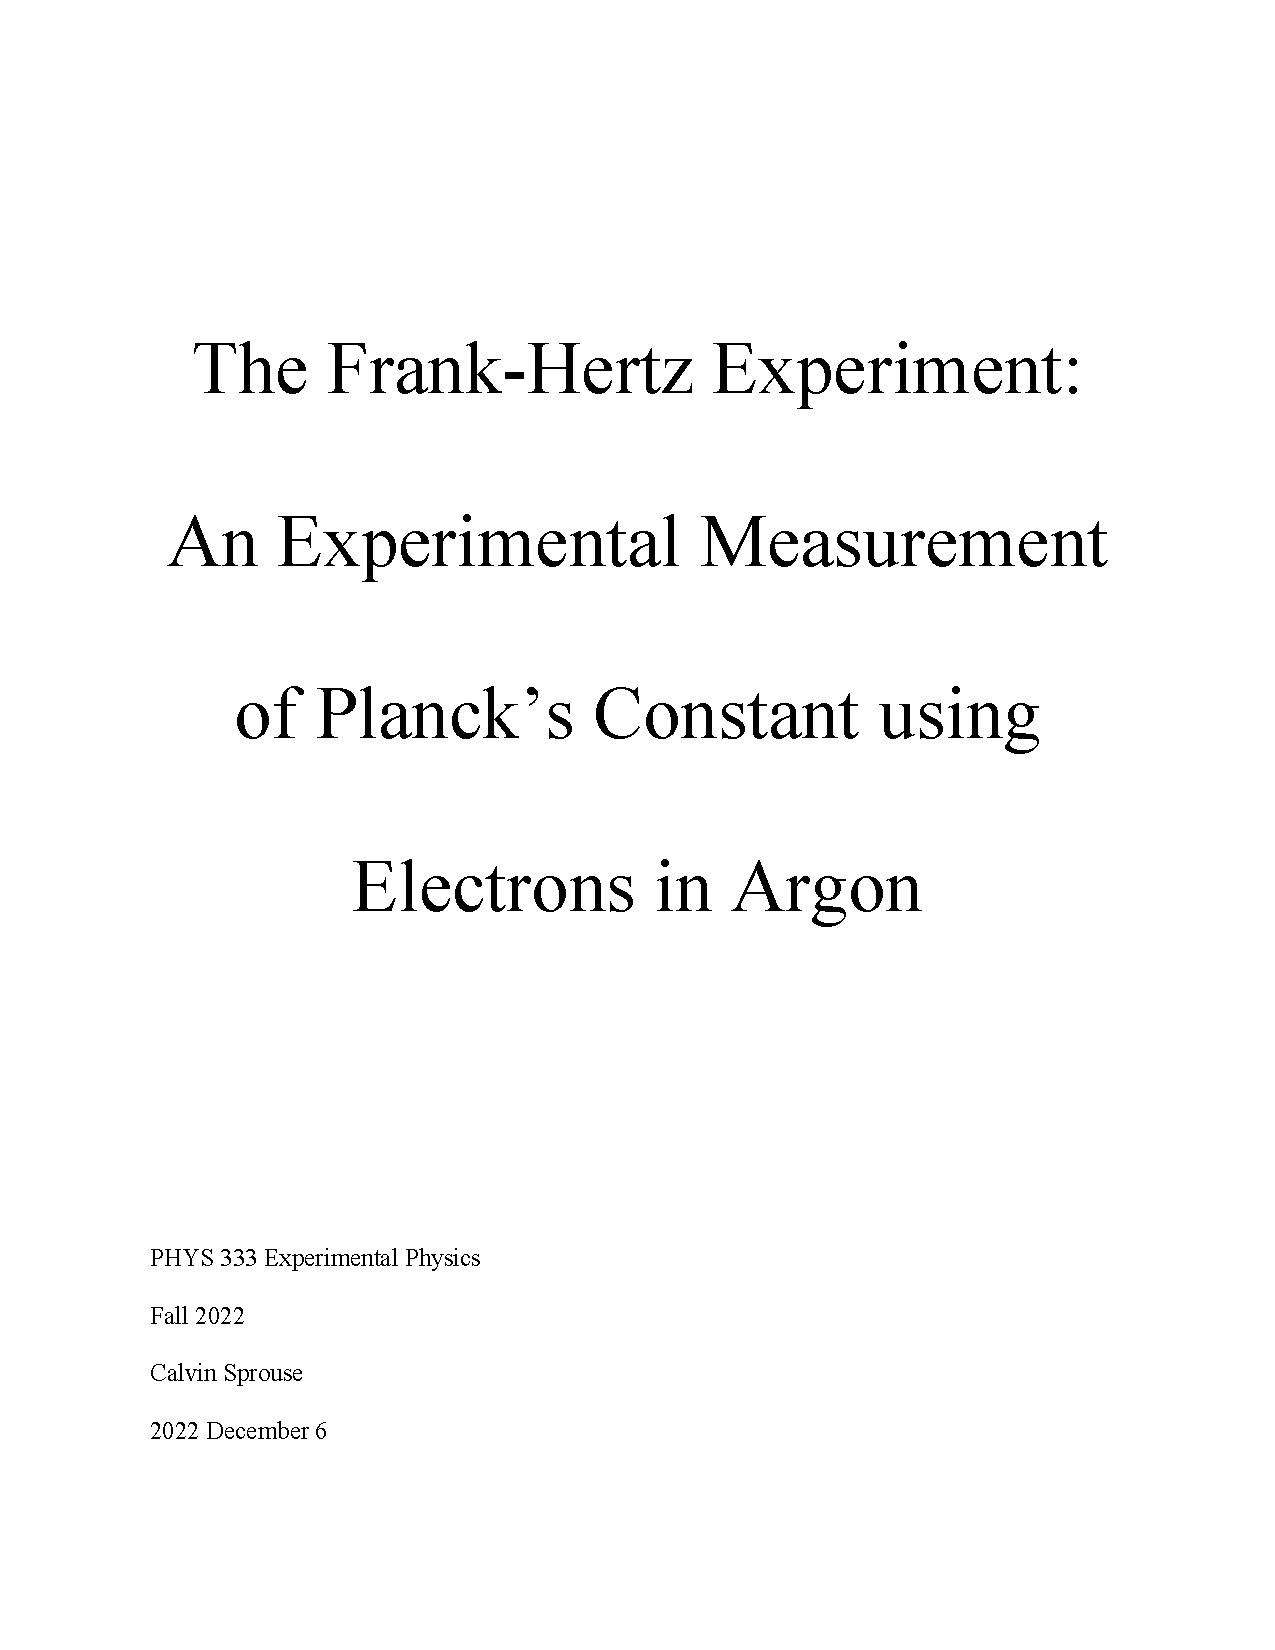
\includepdf[pages=-]{FullReportCalvinSprouse.pdf}
\end{document}
